\documentclass[11pt]{article}
\usepackage{natbib,mybigpackage}
\usepackage{algorithm}
%\usepackage{program}
%\usepackage{algpseudocode}
\usepackage{algorithmic}
\usepackage{listings}


\def\xbf{\mathbf{x}}
\def\zbf{\mathbf{z}}
\def\xibf{\mathbf{\xi}}
\title{MA 226 - Assignment Report 4}
\author{Ayush Sharma\\150123046}
\begin{document}
\titlepage
\newpage

\begin{enumerate}
\item[Q 1]  Simulate 5000 sample of exponential with mean 5.
Draw the histogram and the calculate the mean, maximum and minimum.
(Use R and C/C++)
\end{enumerate}

\noindent{Solution:}  We can write the cumulative density function of Exponential distribution as
$$F_{Exp}(x, \lambda) = (1 - e^{-\lambda x}).$$
To apply inverse transform method we equate $u = (1 - e^{-\lambda x})  \Rightarrow   x = -\frac{1}{\lambda}\log(1 - u)$ where u is an observation from Uniform(0,1).

\begin{algorithm}[H]
\caption{Generating Random number from Exponential distribution}
\begin{algorithmic}[1]
\STATE Generate $U$ from $\mathcal{U}[0,1]$.
\STATE Generate $X$ from the following relation $X = -\frac{1}{\lambda}\log(1 - U)$.
\end{algorithmic}
\end{algorithm}

\noindent{Code for R}

\begin{lstlisting}
genExp<-function(sample, mean) {
  E<-vector(length = sample);

  set.seed(1);
  u<-runif(sample, 0, 1);

  lambda = 1 / mean
  E = ((-1 / lambda) * log(1 - u));

  png("1.png");
  hist(E, breaks = 50, col = "light cyan", plot = TRUE);

  return(c(mean(E), max(E), min(E)));
}

output<-genExp(5000, 5);

cat("The mean, maximum, and minimum are calculated to be", output[1], ",", output[2], ", and", output[3], "respectively.\n");

\end{lstlisting}
\newpage
\noindent{\textbf{Results}:}

The histogram can be shown as :

\begin{figure}[H]
  \centering
  \subfloat[$\xi_{1}$]{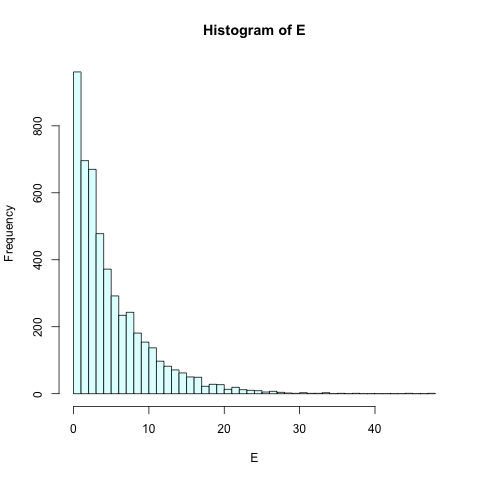
\includegraphics[width=0.7\textwidth]{1.png}}
    \caption{Histogram for n = 5000}
\end{figure}

The mean, maximum, and minimum are calculated to be 5.035687 , 47.87766 , and 0.001002004 respectively.

\newpage

\begin{enumerate}
\item[Q 2] Generate 5000 sample from Gamma with parameter $n = 5$ and $\lambda = 5$.
Draw the histogram and the calculate the mean, maximum and minimum.
(Use R and C/C++)
\end{enumerate}

\noindent{Solution:}  For a Gamma($n$, $\lambda$) random variable, note that because we cannot write an explicit form for the expression of the $F^{-1}$ , it is diffcult to directly apply inverse transform method.\\
However, recall that the sum of independent Exponentials leads us to a Gamma distribution.\\
We can generate from a Gamma distribution by generating $n$ randomnumbers $U_1, U_2, ..., U_n$ and then setting%\hspace{25mm}
$$X = -\frac{1}{\lambda}\log(U_1) - ... -\frac{1}{\lambda}\log(U_n) = -\frac{1}{\lambda}\log(U_1 ... U_n)$$
This works provided $n$ is an integer.

\begin{algorithm}[H]
\caption{Generating Random number from Gamma distribution}
\begin{algorithmic}[1]
\STATE Generate $U_1, U_2, ..., U_n$ from $\mathcal{U}[0,1]$.
\STATE Generate $X$ from the following relation $X = -\frac{1}{\lambda}\log(U_1 ... U_n)$.
\end{algorithmic}
\end{algorithm}

\noindent{Code for R}

\begin{lstlisting}
genGamma<-function(sample, n, lambda) {
  G<-vector(length=sample);

  set.seed(1);

  for (i in 1:sample) {
    u<-runif(n, 0, 1);
    G[i] = prod(u);
  }

  G = (-1 / lambda) * log(G);

  png("2.png");
  hist(G, breaks = 50, col = "light cyan", plot = TRUE);

  return(c(mean(G), max(G), min(G)));
}

output<-genGamma(5000, 5, 5);

cat("The mean, maximum, and minimum are calculated to be", output[1], ",", output[2], ", and", output[3], "respectively.\n");

\end{lstlisting}
\newpage
\noindent{\textbf{Results}:}

The histogram can be shown as :

\begin{figure}[H]
  \centering
  \subfloat[$\xi_{1}$]{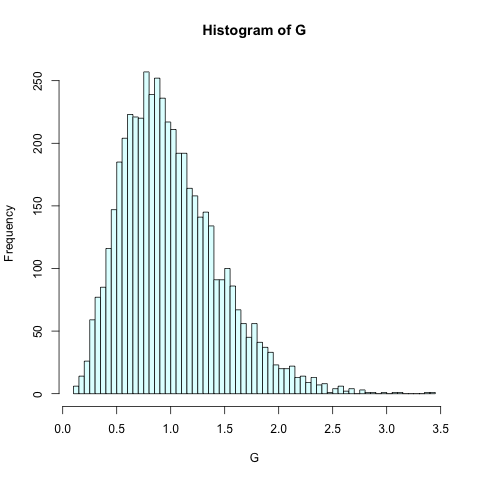
\includegraphics[width=0.7\textwidth]{2.png}}
    \caption{Histogram for n = 5000}
\end{figure}

The mean, maximum, and minimum are calculated to be 1.00498 , 3.447011 , and 0.1211753 respectively.

\newpage

\begin{enumerate}
\item[Q 3] Use the rejection method to generate from $$f(x) = 20x(1-x)^{3}, \hspace{10mm}0 < x < 1.$$
(Use R and C/C++)
\end{enumerate}

\noindent{Solution:}  For generating random number from $f(x) = 20x(1-x)^{3} \hspace{5mm} \{$where $0 < x < 1\}$ by acceptance-rejection method we choose Uniform(0,1) as our candidate distribution. We write the probability density function of Uniform distribution as $g(x) = 1$.\\
We choose c maximizing $\frac{f(x)}{g(x)} = \frac{20x(1-x)^{3}}{1}$.\\
Maximum of c will attain at $x = \frac{1}{4}$ i.e. $c = \frac{135}{64}$.

\begin{algorithm}[H]
\caption{Generating random number from $f(x) = 20x(1-x)^{3} \hspace{5mm} \{$where $0 < x < 1\}$ by acceptance-rejection method}
\begin{algorithmic}[1]
\STATE Generate $U_1, U_2$ from $\mathcal{U}[0,1]$.
%\STATE  
\IF {$U_{2} \leq \frac{f(U_1)}{cg(U_1)} = \frac{20U_1(1-U_1)^{3}}{c}$}
  \STATE  $X = U_1$.
\ELSE
  \STATE  return to step 1.
\ENDIF
\end{algorithmic}
\end{algorithm}

\noindent{Code for R}

\begin{lstlisting}
f<-function(x) {
  return (20 * x * ((1 - x)^3));
}

genF<-function(sample) {

  F<-vector(length = sample);

  c = (135 / 64);

  set.seed(1);

  for (i in 1:sample) {
    repeat {
      u<-runif(2, 0, 1);
      if(u[2] <= (f(u[1])/c)){
        F[i] = u[1];
        break;
      }
    }
  }

  png("3.png");
  hist(F, breaks = 50, col = "light cyan", plot = TRUE);

  return(c(mean(F), var(F), max(F), min(F)));
}

output<-genF(5000);

cat("The mean, variance, maximum, and minimum are calculated to be", output[1], ",", output[2], ",", output[3], ", and", output[4], "respectively.\n");

\end{lstlisting}
\newpage
\noindent{\textbf{Results}:}

The histogram can be shown as :

\begin{figure}[H]
  \centering
  \subfloat[$\xi_{1}$]{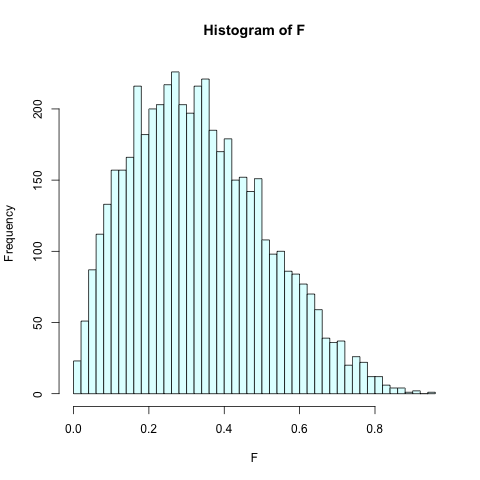
\includegraphics[width=0.7\textwidth]{3.png}}
    \caption{Histogram for n = 5000}
\end{figure}

The mean, variance, maximum, and minimum are calculated to be 0.333445 , 0.03102842 , 0.9569733 , and 0.00372441 respectively.

\end{document}

%#Made by Ayush Sharma#
%#Signed as AShar#